\documentclass{article}
\usepackage[utf8]{vietnam}
\usepackage[12pt]{extsizes}
\usepackage{amsmath,amsfonts,amsthm}
\usepackage{mathrsfs}
\usepackage{enumitem}
\usepackage{geometry}
\usepackage{mathtools}
\usepackage{booktabs}
\usepackage{pgfplots}
\usepackage{amssymb}
\usepackage{array}
\usepackage{multirow}
\usepackage{tabularx}
\usepackage{hyperref}
 \geometry{
 a4paper,
 total={170mm,257mm},
 left=20mm,
 top=20mm,
 }
 \usepackage{graphicx}
 \usepackage{titling}
 \usepackage{listings}
 \title{Lab 3: Làm việc với tiến trình trong Linux
}
\author{23020874 Vũ Hàn Tín}
\date{Ngày 3/5/2025}
 \usepackage{fancyhdr}
\fancypagestyle{plain}{%  the preset of fancyhdr 
    \fancyhf{} % clear all header and footer fields
    \fancyfoot[L]{\thedate}
    \fancyhead[L]{ELT3296 Advanced Programming Techniques}
    \fancyhead[R]{\theauthor}
}
\makeatletter\def\@maketitle{%
\newpage
\null
\vskip 1em%
\begin{center}%
\let \footnote \thanks
  {\LARGE \@title \par}%
  \vskip 1em%
  %{\large \@date}%
\end{center}%
\par
\vskip 1em}
\makeatother
\begin{document}
\maketitle
\section{Lý thuyết}
\subsection{Giới thiệu về tiến trình (process)}
\begin{itemize}
    \item Chương trình (program): là một tập hợp các chỉ dẫn (a set of instructions) được viết bằng ngôn ngữ lập trình dùng để thực thi các
tác vụ (task) và được lưu thụ động trong ổ đĩa (passively stored on disk).
    \item Tiến trình (process): là một trường hợp của chương trình (program) đang được thực thi. Đây là một thực thể (entity) chạy trong bộ nhớ
(runs in memory) và sử dụng tài nguyên hệ thống (utilizes system resource).
\end{itemize}
Chương trình và tiến trình có những đặc điểm khác nhau cơ bản được phân biệt như bảng sau:
\begin{center}
    \begin{table}[h]
        %\centering   % see Mico's comment
        \begin{tabularx}{\linewidth}{|l|X|X|}
        \hline
        \textbf{Tính năng} & \textbf{Chương trình} & \textbf{Tiến trình} \\ \hline
        Định nghĩa & Một tập hợp của các chỉ dẫn (instructions) lưu trữ trong ổ đĩa. & Một chương trình đang được thực thi, chạy trong bộ nhớ (running in memory).  \\ \hline
        Trạng thái & Thụ động (passive, not running). & Chủ động (active). \\ \hline
        Vị trí & Lưu trữ trong ổ đĩa nhưng một file có khả năng thực thi (executable file). &  Tải trong RAM (loaded into RAM) trong quá trình thực thi. \\ \hline
        Tuổi thọ (lifespan) & Vĩnh viễn cho đến khi bị xóa (permanent until deleted). & Tạm thời, tồn tại trong quá trình thực thi (exists while executing). \\ \hline
        Sử dụng tài nguyên (resource usage) & Không dùng CPU, I/O hay bộ nhớ. & Dùng CPU, I/O và bộ nhớ. \\ \hline
        Tính đa dạng (multiplicity) & Một bản copy của chương trình tồn tại trong ổ đĩa. & Nhiều tiến trình của một chương trình có thể chạy đồng thời. \\ \hline
        \end{tabularx}
        \end{table}
\end{center}
Ví dụ: khi ta viết file \verb|hello.c|, lúc đầu đây chỉ là một file text thông thường chứ chưa phải là một chương trình hay tiến trình. Sau khi chạy file trên bằng compiler (\verb|gcc hello.c -o hello| chẳng hạn),
nó tạo ra một file \verb|hello| có khả năng thực thi (executable file). File này là một \textbf{chương trình} (program), một thực thể thụ động (passive entity) được lưu trữ trong ổ đĩa chờ được thực thi. Khi ta
chạy file này bằng câu lệnh \verb|./hello|, hệ điều hành sẽ tải nó vào trong bộ  nhớ (loads it into memory). Lúc này, hệ điều hành sẽ tạo ra \textbf{tiến trình} (process), cung cấp tài nguyên hệ thống (assigning system resources) như CPU time, bộ nhớ và thao tác I/O cho chương trình. 
Khi chương trình thực thi, tiến trình tồn tại trong RAM và thực thi các chỉ dẫn (executes instructions) từ chương trình. 
\\ Chẳng hạn ta viết một file \verb|hello.c| như sau (dùng hàm \verb|getpid()| để trả về PID của tiến trình):
\begin{verbatim}
    #include <stdio.h>
    #include <sys/types.h>
    #include <unistd.h>
    int main(){
        printf("Hello World!\n");
        printf("The PID is %d", getpid()); //Returns PID of a process.
    }    
\end{verbatim}
Chạy chương trình này:
\begin{verbatim}
    Chiaki@mx:~/C
    $ gcc hello.c -o hello | ./hello
    Hello World!
    The PID is 12117
\end{verbatim}
ta thu được kết quả \verb|PID| của tiến trình \verb|./hello| là \verb|12117|. Thế nhưng, nếu ta kiểm tra trong danh sách các tiến trình bằng câu lệnh \verb|grep| để tìm lại \verb|PID|, kết  quả trả về như sau:
\begin{verbatim}
    ps -aux | grep "12117"
    Chiaki     12353  0.0  0.0  78540  1996 pts/2    S+   21:41   0:00 grep 12117
\end{verbatim}
Ta không hề tìm thấy tiến trình có \verb|PID 12117| có trong danh sách (\verb|PID| trả về là \verb|PID| của tiến trình \verb|grep 12117|). Nguyên nhân của vấn đề này là do thời gian
thực thi (execution time) của tiến trình \verb|./hello| quá nhanh nên tiến trình đã kết thúc (terminated) trước khi gọi lệnh \verb|grep|.
\\ Để khắc phục vấn đề này, ta có hai cách đi "đường vòng" như sau:
\begin{enumerate}
    \item  Sử dụng hàm \verb|sleep()| để cho phép chương trình được "trễ" một khoảng thời gian nhất định, ở đây ta sẽ cho phép "trễ" \verb|45s|. Ta viết lại file \verb|hello.c|
như sau:
\begin{verbatim}
    #include <stdio.h>
    #include <sys/types.h>
    #include <unistd.h>
    int main(){
        printf("Hello World!\n");
        printf("The PID is %d", getpid());
        sleep(45); //Waits 45s.
    }    
\end{verbatim}
và chạy lệnh như trên:
\begin{verbatim}
    gcc hello.c -o hello | ./hello
\end{verbatim}
Lúc này thay vì \verb|PID| của tiến trình \verb|./hello| xuất hiện ngay lập tức, nó sẽ xuất hiện sau \verb|45s|, ta mở terminal khác và chạy lệnh \verb|grep| để tìm kiếm, kết quả trả về thu được như sau:
\begin{verbatim}
    $ ps -aux | grep ./hello
    Chiaki     13766  0.0  0.0   2464   912 pts/1    S+   21:54   0:00 ./hello
\end{verbatim}
Ta thu được \verb|PID| của tiến trình \verb|./hello| là \verb|13766|. Sau khi kết thúc \verb|45s|, quay trở lại terminal ban đầu, ta thấy đầu ra lúc này trả về là:
\begin{verbatim}
    $ ./hello                                                                                              
    Hello World!                                                                                           
    The PID is 13766                                                                                                
\end{verbatim}
    \item Sử dụng hàm \verb|scanf()| với vai trò tương tự như hàm \verb|sleep()|, làm "trễ" chương trình bằng cách kiểm soát thời gian thực thi (execution time) với phương thức nhập input từ bàn phím.
\end{enumerate}
Khi một tiến trình được tạo ra, Linux kernel phân phối bộ nhớ (allocates memory) và tổ chức (organizes) nó theo hướng có cấu trúc (structured way). Bộ nhớ sẽ được chia thành các phân đoạn (segments) khác nhau để quản lý hiệu quả code như code thực thi (execution), biến (variables), stack và bộ nhớ động (dynamic memory).
\begin{center}
    \begin{table}[h]
        %\centering   % see Mico's comment
        \begin{tabularx}{\linewidth}{|X|X|X|X|}
        \hline
        \textbf{Phân đoạn} \newline (Segment) & \textbf{Mô tả} & \textbf{Hành vi của bộ nhớ} \newline (Memory behavior) & \textbf{Ví dụ} \\ \hline
        Text (code segment). & Lưu trữ đoạn mã máy của chương trình (instructions). & Chỉ đọc (read-only) để ngăn chặn sửa đổi (prevent modification). &\verb|int main(){...}| \newline Đoạn mã máy (machine code) này được lưu trữ trong phân đoạn \verb|text|. \\ \hline
        Dữ liệu (data segment). & Lưu trữ biến đã khởi tạo toàn cục và tĩnh (initialized global and static variables). & Kích thước cố định, không thay đổi. & \verb|int x = 10;| \newline \verb|static int y = 20;| 2 biến này được lưu trữ trong phân đoạn \verb|data|. \\ \hline
        BBS (block started by symbol). & Lưu trữ biến chưa khởi tạo toàn cục và tĩnh (uninitialized global and static variables) &  Kích thước cố định, không thay đổi. & \verb|int uninit_var;| \newline Lưu trữ trong phân đoạn \verb|BSS|. \\ \hline
        Heap (heap segment) & Lưu trữ bộ nhớ động (dynamic memory) như bộ nhớ được cấp phát bởi các hàm \verb|malloc()|. & Tăng lên (grows upward) về bộ nhớ. & \verb|int *ptr = (int*)|\newline\verb|malloc(sizeof(int))|\newline \verb|;| \newline Lưu trữ trong \verb|heap|.\\ \hline
        Stack (stack segment)& Lưu trữ khung hàm gọi (function call frames), biến bản địa (local variables) và trả về địa chỉ (return addresses). & Giảm đi (grows downward) về bộ nhớ. & \verb|void function()|\newline \verb|{int localVal;...};| \newline Lưu trữ trong \verb|stack|.\\ \hline
        \end{tabularx}
        \end{table}
\end{center}
Kernel không trực tiếp gán (assign) bộ nhớ vật lý (physical memory) RAM cho một tiến trình. Thay vào đó, nó cấp một không gian địa chỉ ảo (virtual address space) hoạt động như một bộ nhớ vật lý trừu tượng (abstraction of physical memory). Mỗi tiến trình có một bộ nhớ ảo (virtual memory) riêng của nó, độc lập với các tiến trình khác.
Đơn vị quản lý bộ nhớ (Memory Management Unit - MMU), cùng với page table (là một cấu trúc dữ liệu được sử dụng bởi bộ nhớ ảo dùng để lưu trữ ánh xạ (mapping) giữa địa chỉ ảo (virtual addresses) và địa chỉ vật lý (physical addresses)), ánh xạ (maps) địa chỉ bộ nhớ ảo (virtual memory address) đến bộ nhớ vật lý thực RAM hay không gian đĩa (disk).
\\ Một tiến trình trong Linux trải qua các giai đoạn khác nhau trong vòng đời (life cycle) gồm: mới (new), chuẩn bị (ready), chạy (running), chờ (waiting/blocked), dừng (terminated).
\begin{enumerate}
    \item New: tiến trình đã được tạo nhưng chưa chạy.
    \item Ready: tiến trình đang đợi (waiting) trong một \verb|queue| cho thời gian CPU (CPU time).
    \item Running: tiến trình hiện tại đang được thực thi (executed) trên CPU.
    \item Blocked (waiting): tiến trình đang chờ một sự kiện (event) như thao tác I/O (I/O operation).
    \item Terminated: tiến trình đã thực thi xong.
\end{enumerate} 
\begin{figure}[h]
    \begin{center}
    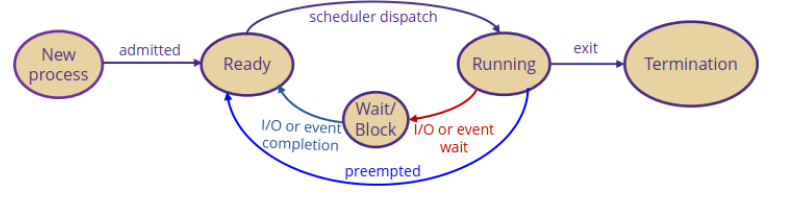
\includegraphics[width=15cm]{3.png}
    \end{center}
    \end{figure}
\subsection{Các system calls đơn giản khi làm việc với tiến trình}
\subsubsection{Tổng quan về các system calls đơn giản}
Ta sẽ tập trung tìm hiểu 4 system calls cơ bản gồm \verb|fork(), execve(), exit(), wait()|, chúng đóng một vai trò cực kì thiết yếu trong quá trình khởi tạo (creation), thực thi (execution), dừng (termination) một tiến trình trong vòng đời (life cycle) của nó.
\begin{itemize}
\item \verb|fork()|: câu lệnh này cho phép một tiến trình cha (parent process) tạo ra một tiến trình con mới (new child process) bằng cách sao chép gần như giống hệt tiến trình cha.
\item \verb|exit(status)|: câu lệnh này cho phép dừng một tiến trình (terminate a process), làm cho toàn bộ tài nguyên (resource) được sử dụng bởi tiến trình ban đầu  được tái phân bổ lại (reallocate) bởi kernel. Đối số (argument) \verb|status| là một số nguyên quyết định trạng thái dừng (termination status) của tiến trình. Sử dụng lệnh \verb|wait()|, tiến trình cha (parent process)
có thể lấy lại trạng thái (status) của nó.
\item \verb|wait(&status)|: câu lệnh này có $2$ mục đích:
\begin{itemize}
    \item Thứ nhất, nếu một tiến trình con (child process) chưa được dừng bởi \verb|exit()|, thì \verb|wait()| sẽ treo thực thi (suspend execution) của tiến trình này cho đến khi một trong các tiến trình con dừng hẳn.
    \item Thứ hai, trạng thái dừng (termination status) của tiến trình con được trả về dưới dạng đối số (argument) \verb|status| của lệnh \verb|wait()|.
\end{itemize}
\item \verb|execve(pathname, argv, envp)|: câu lệnh này tải (loads) một chương trình mới với các đối số \verb|pathname, argument list argv, environment list envp| trong bộ nhớ của tiến trình (process's memory). Chương trình hiện tại bị loại bỏ và các phân đoạn (segments) như \verb|stack, data, heap| đều được khởi tạo hoàn toàn mới
(freshly created) cho chương trình. Thao tác (operation) này tương đương với thực hiện (execing) một chương trình mới.
\end{itemize}
\begin{figure}[h]
    \begin{center}
    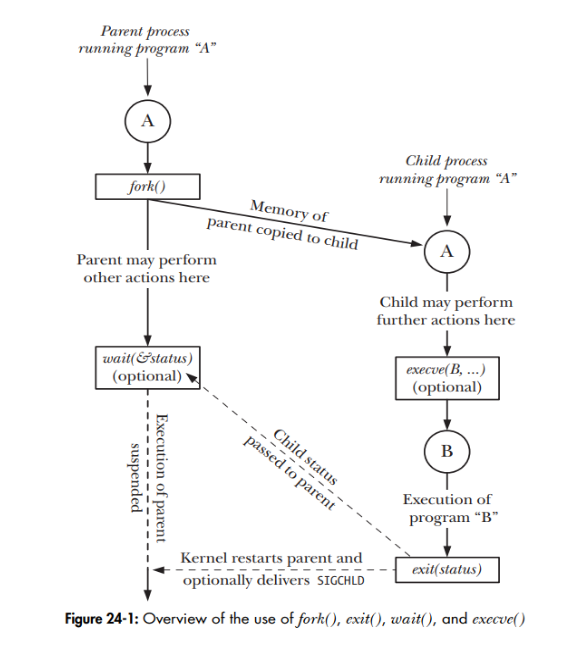
\includegraphics[width=10cm]{31.png}
    \end{center}
    \end{figure}
\subsubsection{Tạo tiến trình mới}
Câu lệnh \verb|fork()| tạo một tiến trình mới, với tiến trình con (child process) gần như giống y hệt bản sao của tiến trình cha (parent process).
Cú pháp của câu lệnh \verb|fork()| như sau:
\begin{verbatim}
    #include <unistd.h>
    pid_t fork(void);
    Returns PID of children on sucess, -1 on error, 0 in successfully created child.
\end{verbatim}
Ví dụ, ta tạo ra tiến trình \verb|./hello| và tiến trình con của nó như sau:
\begin{verbatim}
    #include <stdio.h>
    #include <stdlib.h>
    #include <sys/types.h>
    #include <unistd.h>
    int main(){
        pid_t p = fork();
        if(p<0){
            perror("fork fail");
            exit(1);
        }
        printf("Hello world, process_id(pid) = %d \n", getpid());
        return 0;
    }    
\end{verbatim}
Output thu được là:
\begin{verbatim}
    Hello world, process_id(pid) = 16229 
    Hello world, process_id(pid) = 16230 
\end{verbatim}
2 tiến trình đã được tạo ra, tiến trình cha và con có \verb|PID| tương ứng là \verb|16229| và \verb|16230|. Mỗi một lần gọi câu lệnh \verb|fork()|, tiến trình
đã bị chia nhánh (fork) 2 lần, vậy nếu ta gọi $n$ câu lệnh \verb|fork()| liên tục thì tổng số output sẽ là $2^n$.
\\ Bây giờ ta sử dụng câu lệnh \verb|fork()| để phân biệt giữa tiến trình cha và tiến trình con như sau:
\begin{verbatim}
    #include <stdio.h>
    #include <stdlib.h>
    #include <sys/types.h>
    #include <unistd.h>
    int main(void){
        pid_t pid = fork();
        if(pid == 0){
            printf("Child => PPID: %d PID %d\n", getppid(), getpid());
            exit(0);
        }
        else if(pid > 0){
            printf("Parent => PID: %d\n", getpid());
            printf("Waiting for child process to finish.\n");
            printf("Child process finished.\n");
        }
        else
            printf("Unable to create child process.\n");
        return 0;
    }    
\end{verbatim}
Ta thu được output tương ứng:
\begin{verbatim}
    Parent => PID: 21928
    Waiting for child process to finish.
    Child process finished.
    Child => PPID: 21928 PID 21929    
\end{verbatim}
Một ví dụ phức tạp hơn với hàm \verb|fork()|, với kết quả trả về thu được tiến trình con giờ đã trở thành một tiến trình cha mới:
\begin{verbatim}
    #include <stdio.h>
    #include <unistd.h>
    void main(){
        pid_t pid;
        switch(pid=fork()){
            case -1:
            printf("Error\n");
            case 0:
            printf("Child, PPID: %d, PID: %d\n",getppid(),getpid());
            default:
            printf("Parent, PID: %d\n",getpid());
        }
    }    
\end{verbatim}
Output thu được:
\begin{verbatim}
    Parent, PID: 22473
    Child, PPID: 22473, PID: 22474
    Parent, PID: 22474
\end{verbatim}
\subsubsection{Chờ tiến trình con}
\begin{enumerate}
    \item[A.] Câu lệnh \verb|wait()|:
\\ Khi một tiến trình cha tạo ra tiến trình con, sẽ có lúc cần thiết khi ta cần tiến trình cha thực thi khi và chỉ khi tiến trình con đã thực thi xong. Lệnh
\verb|wait()| có khả năng bắt tiến trình cha phải chờ (wait) cho đến khi tiến trình con hoàn thành và sau đó tiến trình cha mới bắt đầu thực thi trở lại từ sau câu lệnh \verb|wait()|.Một
cách chính xác hơn, ta có thể hiểu câu lệnh này bắt tiến trình cha phải chờ (wait) cho đến khi tiến trình con thay đổi trạng thái (change state) như dừng (terminated), dừng bởi một tín hiệu (stopped by a signal), tiếp
tục thực thi bởi một tín hiệu (resumed by a signal). Cú pháp của câu lệnh này như sau:
\begin{verbatim}
    #include <sys/types.h>
    #include <sys/wait.h>
    pid_t wait(int *status);
\end{verbatim}
Câu lệnh \verb|wait()| chỉ có thể nhận một tham số (parameter) duy nhất có khả năng lưu trữ lại trạng thái thông tin của tiến trình con. Ở ví
dụ dưới đây, ta truyền \verb|NULL| vì ta chưa cần quan tâm đến trạng thái kết thúc của tiến trình con (exit status of child process) và chỉ đơn giản
khiến cho tiến trình cha phải đợi:
\begin{verbatim}
    #include <stdio.h>
    #include <unistd.h>
    #include <sys/wait.h>
    #include <stdlib.h>
    int main(){
        printf("Before fork\n");
        pid_t pid = fork(); 
        if(pid == 0){ //child
            printf("I am child having id %d\n", getpid());
            printf("My parent's id is %d\n", getppid());
        }
        else{ //parent
            wait(NULL);
            printf("My child's id is %d\n",pid);
            printf("I am parent having id %d\n", getpid());
        }
        printf("Common\n");
        return 0;
    }    
\end{verbatim}
Output của chương trình này là:
\begin{verbatim}
    $ ./wait                                                                                                                                                                                                       
    Before fork                                                                                                                                                                                                    
    I am child having id 51237                                                                                                                                                                                     
    My parent's id is 51236                                                                                                                                                                                        
    Common                                                                                                                                                                                                         
    My child's id is 51237                                                                                                                                                                                         
    I am parent having id 51236                                                                                                                                                                                    
    Common  
\end{verbatim}
Chương trình \verb|wait.c| thực thi (execute) tiến trình con trước tiến trình cha, ngược lại nếu ta comment câu lệnh \verb|wait(NULL)| thì ouput như sau:
\begin{verbatim}
    Before fork      
    My child's id is 51468                                                                                                                                                                                                                                                                                                                                                       
    I am parent having id 51467                                                                                                                                                                   
    Common                                                                                                                             
    I am child having id 51468  
    My parent's id is 1                                                                                                                                                                                                                                                                                                                                                                   
    Common
\end{verbatim}
Chương trình lúc này đã thực thi tiến trình cha trước, rồi mới đến tiến trình con. Thế nhưng ta dễ dàng nhận thấy \verb|My parent's id is 1| không phải là ID của tiến trình cha.
Lý do bởi vì các câu lệnh \verb|getpid(), getppid()| hoạt động như lệnh \verb|enQueue()|, nên ta phải gọi câu lệnh \verb|getppid()| trước rồi mới đến \verb|getpid()| theo thứ tự
FIFO. Thế nên để chương trình chạy đúng (không có lệnh \verb|wait(NULL)|), ta cần phải đảo thứ tự trong khối lệnh của tiến trình con như sau:
\begin{verbatim}
    printf("My parent's id is %d\n", getppid());                                                                                                                                                           
    printf("I am child having id %d\n", getpid());
\end{verbatim}
Khi ta muốn câu lệnh \verb|wait()| trả về giá trị (returns value), nó có thể trả về \verb|PID| của tiến trình con đã bị dừng (terminated child process) 
hoặc \verb|-1| nếu có lỗi xảy ra (error occurs). Ví dụ:
\begin{verbatim}
    #include <stdio.h>                                                                                                                                                                                             
    #include <unistd.h>                                                                                                                                                                                            
    #include <sys/wait.h>                                                                                                                                                                                          
    #include <stdlib.h>                                                                                                                                                                                            
    int main(){                                                                                                                                                                                                    
        int status;                                                                                                                                                                                                
        if(fork() == 0){                                                                                                                                                                                           
            printf("Hello from children\n");                                                                                                                                                                       
            sleep(30);                                                                                                                                                                                             
            exit(0);                                                                                                                                                                                               
        }                                                                                                                                                                                                          
        else{                                                                                                                                                                                                      
            printf("Hello from parent\n");                                                                                                                                                                         
            pid_t pid = wait(&status);                                                                                                                                                                             
            printf("Child process terminated has ID: %d",pid);                                                                                                                                                     
        }                                                                                                                                                                                                          
        return 0;                                                                                                                                                                                                  
    }
\end{verbatim}
Lúc này chương trình sẽ in ra \verb|PID| của tiến trình con sau \verb|30s| chờ (sleep) là \verb|55370|, kiểm tra lại bằng câu lệnh \verb|ps -aux|, ta  thấy kết quả hoàn toàn trùng khớp.
    \item[B.] Câu lệnh \verb|waitpid()|: 
\\ Câu lệnh \verb|waitpid()| là một phiên bản cải tiến hơn của \verb|wait()|, được thiết kế để cung cấp thêm quyền kiểm soát (control) khi chờ (wait) tiến trình con. Nó
cho phép lựa chọn tiến trình con để chờ (wait), thực hiện (perform) non-blocking waits và giám sát (monitor) tiến trình con đổi trạng thái (change state). Cú pháp của câu lệnh này như sau:
\begin{verbatim}
    #include <sys/wait.h>
    pid_t waitpid(pid_t pid, int *status, int options);
    return PID of waited-for child, 0 in non-blocking mode, -1 on error
\end{verbatim}
Các tham số (parameter) truyền vào gồm:
\begin{itemize}
    \item \verb|pid|: xác định (spectifies) xem tiến trình con nào sẽ được tiến trình cha chờ.
    \begin{itemize}
        \item \verb|pid > 0|: chờ một tiến trình con với ID đã xác định.
        \item \verb|pid == 0|: chờ tất cả tiến trình con trong cùng một nhóm tiến trình (same process group).
        \item \verb|pid < -1|: chờ tất cả các tiến trình con trong cùng một nhóm tiến trình được xác định bởi \verb|-pid|.
        \item \verb|pid == -1|: chờ tất cả các tiến trình (tương đương với \verb|wait()|).
    \end{itemize}
    \item \verb|status|: con trỏ trỏ tới số nguyên lưu giữ thông tin về tiến trình con bị dừng (terminated).
    \item \verb|options|: tùy chọn bổ sung cho điều khiển hành vi (behavior control).
    \begin{itemize}
        \item \verb|WUNTRACED|: trả lại trạng thái (returns status) khi tiến trình con bị dừng bởi một tín hiệu.
        \item \verb|WCONTINUED|: trả lại trạng thái khi tiến trình con đã bị dừng (stopped signal) được khôi phục lại.
        \item \verb|WNOHANG|: thực hiện non-blocking check (\verb|return 0| nếu không có tiến trình con nào chuyển trạng thái ở đây).
    \end{itemize}
\end{itemize}
\end{enumerate}
Ví dụ
\begin{verbatim}
    #include <stdio.h>
    #include <unistd.h>
    #include <sys/wait.h>
    #include <stdlib.h>
    int main(){
        int status;
        pid_t child_pid = fork();
        if(child_pid > 0){
            waitpid(child_pid, &status, 0);
            printf("I am the parent\n");
        }
        else if(child_pid == 0){
            printf("I am the child\n");
        }
        else{
            printf("Fork failed\n");
        }
        return 0;
    }
\end{verbatim}
\subsubsection{Thực thi chương trình}
Các câu lệnh thuộc họ \verb|exec()| tải một chương trình mới (loads a new program) vào bộ nhớ tiến trình (process's memory), thay thế chương trình hiện tại.
Các cấu trúc dữ liệu của chương trình cũ như \verb|stack, queue, heap| đều bị loại bỏ. Chương trình mới bắt đầu được thực thi từ hàm \verb|main()| sau một khoảng thời gian khởi tạo.
Cú pháp tổng quát của các câu lệnh này như sau:
\begin{verbatim}
    #include <unistd.h>
    int exec(const char *pathname, char *const argv[], char *const envp[]);
    Returns -1 on error, never return on success.
\end{verbatim}
Các tham số (parameter) được truyền (pass) vào cụ thể gồm:
\begin{center}
    \begin{tabular}{ | l |l| } 
      \hline
      pathname & Can be relative or absolute path \\ 
      \hline
      argv[] (command lines argument) & Spectifies arguments passed to new program  \\ 
      \hline
      envp[] (environment variables) & Defines the environment for the new program \\ 
      \hline
    \end{tabular}
    \end{center}
Ví dụ: để cho đơn giản ta sử dụng câu lệnh \verb|execvp()| với 2 tham số đầu vào như sau:
\begin{verbatim}
    // Write EXEC.c file first
    #include <stdio.h>
    #include <unistd.h>
    int main(){
        int i;
        printf("I am EXEC.c called by execvp()");
        return 0;
    }
    // Write execDemo.c file later
    #include <stdio.h>
    #include <unistd.h>
    #include <stdlib.h>
    int main(){
        char *argv[]  ={ "./EXEC", NULL}; // argv[0] contains program name 
        execvp(argv[0], argv);            // and must be NULL terminated
        printf("Ending----");
        return 0;
    } 
    // And then, run these commands on bash
    gcc execDemo.c -o execDemo
    ./execDemo
    //Result
    I am EXEC.c called by execvp()
\end{verbatim}
Ở đây ta có thể thấy câu lệnh \verb|execvp()| đã chạy một chương trình C (\verb|EXEC.c|) bằng cách sử dụng một chương trình khác (\verb|execDemo.c|),
và dòng \verb|Ending----| không xuất hiện do kể từ khi \verb|execvp()| được gọi, chương trình \verb|execDemo.c| đã bị 
chương trình \verb|EXEC.c| thay thế hoàn toàn. Cú pháp của lệnh \verb|execvp()| này là:
\begin{verbatim}
    int execvp (const char *file, char *const argv[]);
\end{verbatim}
\subsubsection{Dừng tiến trình}
Câu lệnh \verb|exit()| được sử dụng để dừng tiến trình (terminate), cú pháp của nó rất đơn giản như sau:
\begin{verbatim}
    #include <unistd.h>
    void exit(int status); // Doesn't return anything
\end{verbatim}
Câu lệnh này chỉ cần  truyền vào một tham số trạng thái (status parameter) duy nhất với quy tắc sau:
\begin{itemize}
    \item \verb|0|: chương trình đã được thực thi (executed) thành công.
    \item \verb|1|: chương trình thực thi (executed) thất bại.
\end{itemize}
Ví dụ:
\begin{verbatim}
    #include <stdio.h>
    #include <stdlib.h>
    #include <fcntl.h>
    int main(){
        int fd = open("./fourier.pdf", O_RDONLY);
        if(fd < 0){
            perror("open");
            exit(1); // Or EXIT_FAILURE
        }
        printf("Open successfully");
        exit(0); // Or EXIT_SUCCESS
    }
\end{verbatim}
Kết quả trả về:
\begin{verbatim}
    open: No such file or directory // Only display perror("open")
\end{verbatim}
\subsection{Tương tác liên tiến trình (Interprocess Communication)}
\subsubsection{Tương tác bằng tín hiệu (signal)}
Tín hiệu là các thông điệp (messsages) nhỏ thông báo cho tiến trình khi có sự kiện (events) diễn ra ở trong hệ thống. Chúng là một phương thức
để cho các tiến trình tương tác với nhau, và một tiến trình có thể nhận tín hiệu ở bất kì thời điểm nào. Tín hiệu có thể được tạo ra từ kernel, tiến trình khác hoặc chính nó. Cú pháp của câu lệnh này là:
\begin{verbatim}
    #include <signal.h>
    int kill(pid_t pid, int sig); //pid of the target process.
\end{verbatim}
Các tham số (parameter) truyền vào cụ thể gồm:
\begin{itemize}
    \item \verb|pid > 0|: tín hiệu được gửi đến PID của tiến trình đích (target process).
    \item \verb|pid == 0|: tín hiệu được gửi đến tất cả tiến trình.
    \item \verb|pid == -1|: tín hiệu được gửi đến tất cả tiến trình ngoại trừ tiến trình khởi tạo.
    \item \verb|pid < -1|: tín hiệu được gửi đến tất cả các tiến trình \verb|-pid|.
\end{itemize}
Để cho đơn giản, ta mặc định giá trị của \verb|int sig = 9| (tương ứng với tín hiệu \verb|SIGKILL|). Ví dụ:
\begin{verbatim}
    #include <stdio.h> //First, write a new loop.c file and run it.
    #include <unistd.h>
    #include <stdlib.h>
    int main(){
        while(1){
            printf("The process's PID is %d\n", getpid());
        }
        return 0;
    }
    // We have the PID is 41302 (or other), and we write another program to kill it.
    // Then, write a new kill.c file and run.
    #include <signal.h>
    int main(){
        pid_t pid = 41302; // ./loop PID
        kill(pid, SIGKILL);
        return 0;
    }
    Final output: successfully break infinite loop with SIGKILL
    ...
    The process's PID is 41302
    The process's PID is 41302Killed    
\end{verbatim}
\subsubsection{Tương tác bằng pipe}
Pipe là một cơ chế một chiều tương tác giữa các tiến trình cho phép dữ liệu chảy (flows) giữa producer (writing process) và
consumer (reading process). Pipe đóng vai trò như một bộ đệm (buffer) giữa các tiến trình. Producer viết data vào trong pipe và consumer đọc data từ pipe.
\begin{figure}[h]
    \begin{center}
    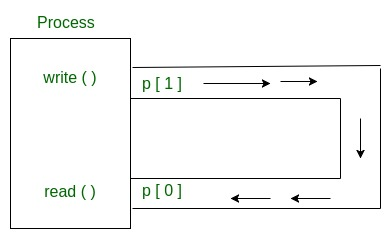
\includegraphics[width=10cm]{pipe.jpg}
    \end{center}
    \end{figure}
\\Cú pháp của câu lệnh này như sau:
\begin{verbatim}
    #include <unistd.h>
    int pipe(int fd[2]);
    Returns 0 on sucess, -1 on failure.
\end{verbatim}
với tham số \verb|fd[2]| là một mảng kiểu nguyên với \verb|fd[0]| được đọc bởi consumer và \verb|fd[1]| được viết bởi
producer. Ví dụ:
\begin{verbatim}
    #include <stdio.h>
    #include <string.h>
    #include <unistd.h>
    #include <sys/wait.h>
    #include <stdlib.h>
        int main(){
        int fd[2];
        char buffer[50];
        if(pipe(fd) == -1){
            perror("Pipe failed");
            exit(1);
        }
        if(fork() > 0){ //Parent process (producer)
            close(fd[0]);
            char message[] = "Hello from parent";
            write(fd[1], message, strlen(message) + 1);
            close(fd[1]);
        }
        else{
            close(fd[1]); //Child process (consumer)
            read(fd[0], buffer, sizeof(buffer));
            printf("Child received %s\n", buffer);
            close(fd[0]);
        }
        return 0;
    }
    //Output: Child received Hello from parent as we expected.
\end{verbatim}
\section{Thực hành}
\subsection{Exercise 1:}
\begin{verbatim}
    #include <stdio.h>
    #include <unistd.h>
    #include <stdlib.h>
    int main(){
        pid_t pid = fork();
        if(pid > 0){ //Parent doesnt have to wait for the child process
            printf("This is parent process\n");
            printf("Parent process PID is %d\n", getpid());
            printf("Children process PID is %d\n", pid);
            exit(0);
        }
        else if(pid == 0){
            printf("This is child process\n");
            printf("Parent and child process PID are: %d %d\n", getppid(), getpid());
            exit(0);
        }
        else{
            perror("fork");
            exit(1);
        }
        return 0;
    }
    /* Output:
    This is parent process
    Parent process PID is 54249
    Children process PID is 54250
    This is child process
    Parent and child process PID are: 54249 54250 */  

    #include <stdio.h>
    #include <unistd.h>
    #include <stdlib.h>
    #include <sys/wait.h>
    int main(){
        pid_t pid = fork();
        if(pid > 0){ //Parent MUST wait for the child process
            wait(NULL);
            printf("This is parent process\n");
            printf("Parent process PID is %d\n", getpid());
            printf("Children process PID is %d\n", pid);
            exit(0);
        }
        else if(pid == 0){
            printf("This is child process\n");
            printf("Parent and child process PID are: %d %d\n", getppid(), getpid());
            exit(0);
        }
        else{
            perror("fork");
            exit(1);
        }
        return 0;
    }    
    /* Output:
    This is child process
    Parent and child process PID are: 54364 54365
    This is parent process
    Parent process PID is 54364
    Children process PID is 54365 */
\end{verbatim}
\subsection{Exercise 3:}
\begin{verbatim}
    #include <stdio.h>
    #include <unistd.h>
    #include <stdlib.h>
    #include <sys/wait.h>
    #include <dirent.h>
    #include <string.h>
    int main(){
        pid_t pid = fork();
        if(pid > 0){  
            wait(NULL);
            exit(0);
        }
        else if(pid == 0){
            char buffer[1000] = "/home";
            DIR *dp = opendir(buffer);
            if(dp==NULL){
            perror("open dir");
            exit(EXIT_FAILURE);
            }
            struct dirent *entry;
            while((entry=readdir(dp))!=NULL){
            printf("Entry: %s\n", entry->d_name);
            }
            exit(0);
        }
        else{
            perror("fork");
            exit(1);
        }
        return 0;
    }
    /* Output
    Entry: .
    Entry: Chiaki
    Entry: ..
    */  
\end{verbatim}
\subsection{Exercise 5:}
\begin{verbatim}
    #include <stdio.h>
    #include <string.h>
    #include <unistd.h>
    #include <stdlib.h>
    #include <sys/wait.h>
    int main(){
        int fd1[2];
        char buffer1[50];
        if(pipe(fd1) == -1){
            perror("Pipe failed");
            exit(1);
        }
        if(fork() == 0){
            close(fd1[0]);
            char message1[] = "Hello from child";
            write(fd1[1], message1, strlen(message1) + 1);
            close(fd1[1]);
        }
        else{
            close(fd1[1]);
            read(fd1[0], buffer1, sizeof(buffer1));
            printf("Received from child: %s\n", buffer1);
            close(fd1[0]);
        }
    
        int fd2[2];
        char buffer2[50];
        if(pipe(fd2) == -1){
            perror("Pipe failed");
            exit(1);
        }
        if(fork() > 0){
            close(fd2[0]);
            char message2[] = "Hello from parent";
            write(fd2[1], message2, strlen(message2) + 1);
            close(fd2[1]);
        }
        else{
            close(fd2[1]);
            read(fd2[0], buffer2, sizeof(buffer2));
            printf("Received from parent: %s\n", buffer2);
            close(fd2[0]);
        }
        return 0;
    }
    /* Output
    $ ./pipe
    Received from child: Hello from child
    Received from parent: Hello from parent
    */
\end{verbatim}
\end{document}